\chapter{Design}
% introduction about the network stack?

\section{Overview}
The networking stack introduced in this thesis is implemented in the C\# 
programming language with SME. The aim of its design is to capacitate performance,
flexibility, and ease of use. In this chapter, the design principles are 
described, the architecture of the solution is outlined, and the components are
outlined.


\subsection{Design principles}
As briefly mentioned in the introduction, the proposed network stack is to 
provide an alternative to the existing proprietary network offloading engines.
While the main goal of this thesis is to research and study the suitability of 
SME for implementing a TCP/IP stack on an FPGA, there are many other aspects of the 
system to be studied.\\
% TODO 
% * support for various FPGAs
% * extensible network stack (not locked to few protocols)
% * firewall

\subsection{Initial requirements}
Following our design principles, initial requirements and goals for the 
networking stack are set so that these can be tested and improved upon. 
\begin{itemize}
\item \textbf{Essential protocols only}\\
Considering that the SME project is still fairly early in its development, and considering 
the sheer number of protocols in the internet protocol suite, the networking 
stack in this thesis is to support only the absolutely essential protocols 
required to provide the users with a meaningful interface to the internet.
These protocols should be picked such that the system can provide the end-user
with a network data-stream, which can transport information to and from a remote
computer.\\
The initial protocols chosen may be implemented and supported partially, but 
they must not deviate from the standard specifications. 

\item \textbf{Support an interface for the end-user}\\
The system must be controlled by an end-user on the FPGA. Such an interface is 
very unique in its own way, compared to standard software interfaces, like the 
ones defined in the POSIX collection of specifications. By supporting such an
external interface gains insight in the way such a networking stack will be used,
and which measures must be taken in order to provide the best possible integration
and performance considerations.

\item \textbf{Independent of underlying physical hardware}\\
By using SME, the underlying hardware description language code can be abstracted
away from the actual implementation. This will later provide developers to easily
modify and tweak the networking stack without having to consider the target 
hardware.\\
Likewise, the networking stack may not rely on using a certain physical layer hardware,
and must be designed to be independent of the underlying hardware used for the 
physical connections. This will ensure that the target hardware can easily 
swap between physical connectors, such as going from ethernet cables to wireless,
or even another FPGA.
\end{itemize}

\section{The architecture}
\subsection{Initial design}

\begin{figure}
    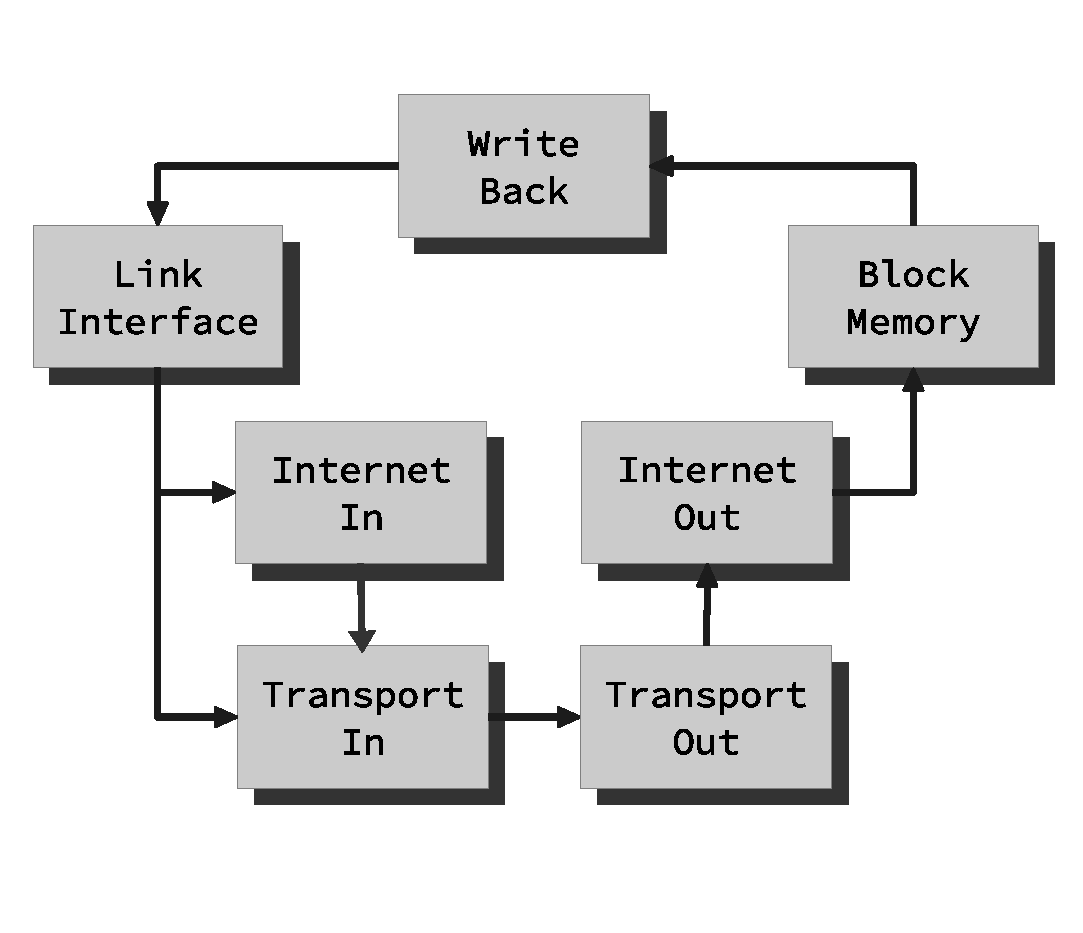
\includegraphics[scale=0.45]{design/design_0.eps}
    \caption{The initial design}
    \label{fig:initial_design}
\end{figure}

The initial architecture focused heavily on the input from the link interface, 
and how to minimize the latency from the source data-stream to its respective
layer handler.\\
In the initial design, figure \ref{fig:initial_design}, the link interface, which
provides the raw byte-stream from the network, is connected to all of the input
parsing layers. The layers are connected in the order in which a network frame 
is parsed; link- to internet- to transport-layer. This approach aims to utilize
the fact that the layers can act immediatelly upon the packets received directly
from the source, as well as easing the logic required to buffer the data across
the layers.\\
This design starts by the Link Interface sending one byte at a time through its bus. 
The \texttt{Link In} will parse the first header, and signal the next layer upon completion.
\texttt{Internet In} will then start to listen on the \texttt{Link Interface} bus
and, using the information from \texttt{Link In}, parse the internet header 
accordingly. The same procedure would be applied to the connection between 
\texttt{Internet In} and \texttt{Transport In}.\\
When data is to be sent to the internet, the network frame would be built bottom
up from the transport layer through internet to the link layer.

\subsubsection{The issues}
The issues quickly surfaced during the implementation of the design. Although 
the interconnect from the \texttt{Link Interface} to all the subsequent layers
in parallel promised negligible latency, it came with a great cost to the solution:
\begin{itemize}
\item \textbf{Process under-utilization}\\
Since each "in" process has to wait for the previous layer to signal when to 
start listening on the data-bus, the layers would in average only be active a third
of the time. Since each layer has very little information about the states of 
the other layers, it would become a challenge to get any other work done during
these phases.\\
For example, it would be an immense challenge to coordinate an ICMP reply on a 
faulty packet in the \texttt{Internet In}.

\item \textbf{IPv4 fragmentation and out of order TCP packets}\\
The chaotic nature of internet routing might cause packets to come out of order,
or even get fragmented along the way. Since each layer parses the packet immediatelly
as it is written to the bus, it became a challenge for the layers to figure out 
what to do. On IPv4 fragmentation, if the second half of a dataframe arrived 
first, the Transport header would not be available to the Transport layer. 
Although IPv4 fragmentation is an increasingly rare phenomenon, the network 
design is not able to handle the situation well.  

% \item \textbf{Control and logic flow} \\
% Although the layers take turns to parse the incoming byte-stream, the design 
% handles the whole packets at once.  

\item \textbf{Redundant Link layer}\\
While the Link layer is an essential part of the Internet Protocol Suite, it did 
not fit well with the functionality of the rest of the stack. 
Most network interfaces are equipped with buffers, on which integrated circuits
perform operations such as error check using cyclic redundancy check, de-noising,
timeslot management, etc. 
Likewise, the Pmod NIC100 Ethernet interface has built-in controller with 
internal memory suited for buffering the incoming packets\cite{microchip_enc424j600}.
This memory, apart from the cyclic redundancy check, can be used as the initial
step for parsing the packet, and only send the datagram to the stack.

\end{itemize}

\section{Link}

\section{Internet}

\section{Transport}

\section{Interface}

